% This LaTeX was auto-generated from MATLAB code.
% To make changes, update the MATLAB code and export to LaTeX again.

\documentclass{article}

\usepackage[utf8]{inputenc}
\usepackage[T1]{fontenc}
\usepackage{lmodern}
\usepackage{graphicx}
\usepackage{color}
\usepackage{hyperref}
\usepackage{amsmath}
\usepackage{amsfonts}
\usepackage{epstopdf}
\usepackage[table]{xcolor}
\usepackage{matlab}
\usepackage[paperheight=795pt,paperwidth=614pt,top=72pt,bottom=72pt,right=72pt,left=72pt,heightrounded]{geometry}

\sloppy
\epstopdfsetup{outdir=./}
\graphicspath{ {./hw11_media/} }

\begin{document}

\title{Homework 11:}
\author{Matthew Luyten\\
ECE6250}

\maketitle

\matlabheading{Problem 11.1}

\vspace{1em}
\begin{par}
\begin{flushleft}
This week, we learned about common algorithms in data science and their applications to DSP. We covered
steepest descent, which is a clever "blunt instrument" approach to solving the linear inverse problem.
Functionally, it wanders around in the solution space and measures its residual error. In order to find
an optimal solution, the algorithm "wanders" in the direction of the smallest residual.
We also covered the conjugate gradient descent algorithm, which improves on steepest descent by cleverly 
applying some properties of orthogonality.
\end{flushleft}
\end{par}

\vspace{1em}
\begin{par}
\begin{flushleft}
In addition, we learned about kSVD and PCA, which are sparse representation and dimensionality reduction 
tools, These are invaluable when dealing with the large datasets that are ubiquitous in real life 
applications. 
\end{flushleft}
\end{par}

\vspace{1em}
\begin{par}
\begin{flushleft}
These topics serve as a bookend to semester of learning advanced DSP. Thanks for everything!
\end{flushleft}
\end{par}

\newpage

\matlabheading{Problem 11.3}

\begin{par}
\begin{flushleft}
Note: I added an initial guess (x0) because it is impossible to ascertain the dimension of x from the function handle H.
\end{flushleft}
\end{par}

\begin{matlabcode}
function [x, iter] = sdsolve(H, b, x0, tol, maxiter)
    x = x0;
    r = b - H(x);
    for iter = 1:maxiter
        if norm(r)/norm(b) < tol
            break;
        end
        q = H(r);
        a = (r'*r)/(r'*q);
        x = x + a * r;
        if mod(iter, 50) == 0
            r = b - H(x);
        else
            r = r - a*q;
        end
    end
end
\end{matlabcode}

\begin{par}
\begin{flushleft}
Provided image convolution function:
\end{flushleft}
\end{par}

\begin{matlabcode}
% imconv.m
%
% Convolves a square image with a square kernel
%
% Written by: Justin Romberg, Georgia Tech
% Created: 11/17/2011

function Y = imconv(X, W)
N = size(X, 1);
K = size(W, 1);
Y = ifft2(fft2(X,N+K-1,N+K-1).*fft2(W,N+K-1,N+K-1));
end
\end{matlabcode}

\begin{par}
\begin{flushleft}
Provided image convolution inverse function:
\end{flushleft}
\end{par}

\begin{matlabcode}
% imconv_transpose.m
%
% Convolves a square image with the "flipped" version of the square kernel,
% and takes the middle part.
%
% This is the adjoint of imconv.m.
%
% Written by: Justin Romberg, Georgia Tech
% Created: 11/17/2011

function V = imconv_transpose(Y, W)
M = size(Y, 1);
K = size(W, 1);
N = M - K + 1;
Vu = ifft2(fft2(Y,N+2*K-2,N+2*K-2).*fft2(rot90(W,2) ,N+2*K-2,N+2*K-2));
V = Vu(K:N+K-1,K:N+K-1);
end
\end{matlabcode}

\begin{par}
\begin{flushleft}
The steepest descent algorithm recovers the original image within a relative error of ${10}^{-4}$ in 599 steps.
\end{flushleft}
\end{par}

\begin{matlabcode}
load imagedeconv_data

A = @(z) reshape(imconv(reshape(z,N,N), W), (N+K-1)^2, 1);
At = @(z) reshape(imconv_transpose(reshape(z, N+K-1, N+K-1), W), N^2, 1);
AtA = @(z) At(A(z));

y = reshape(Y, (N+K-1)^2, 1);

imagesc(Y); colormap("gray"); title("Convolved Image");
\end{matlabcode}
\begin{center}
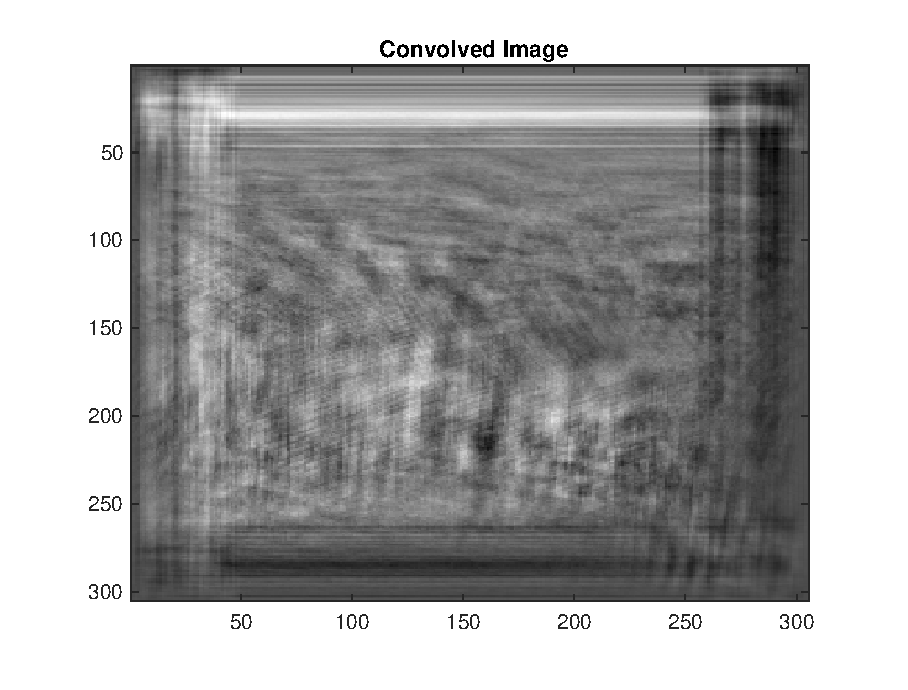
\includegraphics[width=\maxwidth{56.196688409433015em}]{figure_0.eps}
\end{center}
\begin{matlabcode}
[x, iter] = sdsolve(AtA, At(y), zeros(N*N, 1), 10^-4, 10000);

x_sc = reshape(x, N, N);
imagesc(x_sc); colormap("gray"); title("Recovered Image (sdsolve)");
\end{matlabcode}
\begin{center}
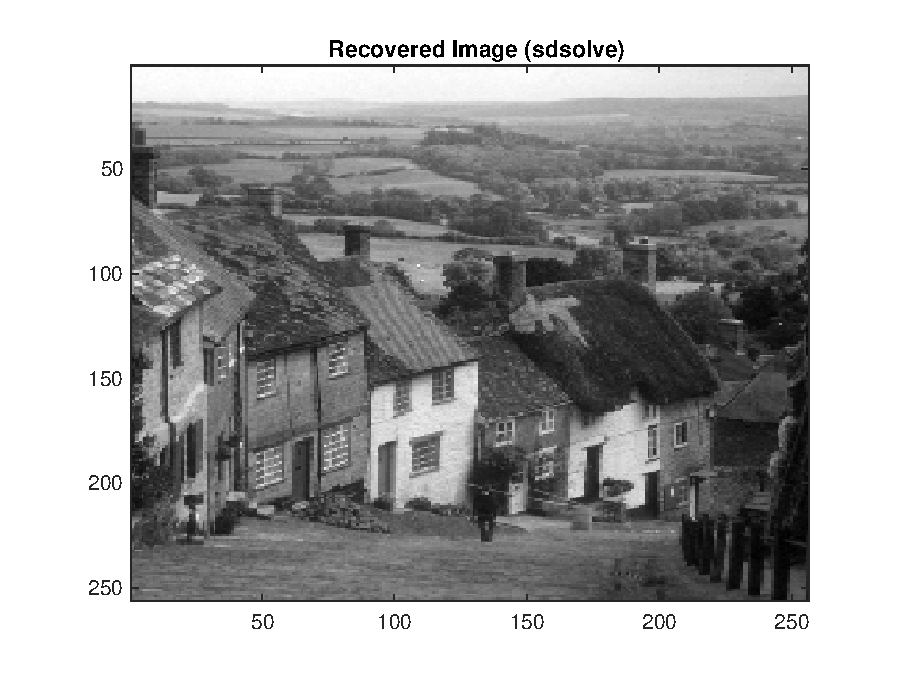
\includegraphics[width=\maxwidth{56.196688409433015em}]{figure_1.eps}
\end{center}
\begin{matlabcode}
fprintf("Original image found in %d steps w/ steepest descent\n", iter);
\end{matlabcode}
\begin{matlaboutput}
Original image found in 599 steps w/ steepest descent
\end{matlaboutput}

\newpage

\matlabheading{Problem 11.4}

\begin{par}
\begin{flushleft}
Note: I added an initial guess (x0) because it is impossible to ascertain the dimension of x from the function handle H.
\end{flushleft}
\end{par}

\begin{matlabcode}
function [x, iter] = cgsolve(H, b, x0, tol, maxiter)
    x = x0;
    r = b - H(x);
    d = r;
    for iter = 1:maxiter
        if norm(r)/norm(b) < tol
            break;
        end
        a = (r'*r)/(d'*H(d));
        x = x + a * d;
        if mod(iter, 50) == 0
            r1 = b - H(x);
        else
            r1 = r - a*H(d);
        end
        beta = (r1'*r1)/(r'*r);
        d = r1 + beta * d;
        r = r1;
    end
end
\end{matlabcode}

\begin{par}
\begin{flushleft}
The conjugate gradient descent algorithm recovers the original image within a relative error of ${10}^{-4}$ in 77 steps.
\end{flushleft}
\end{par}

\begin{matlabcode}
load imagedeconv_data

A = @(z) reshape(imconv(reshape(z,N,N), W), (N+K-1)^2, 1);
At = @(z) reshape(imconv_transpose(reshape(z, N+K-1, N+K-1), W), N^2, 1);
AtA = @(z) At(A(z));

y = reshape(Y, (N+K-1)^2, 1);

[x, iter] = cgsolve(AtA, At(y), zeros(N*N, 1), 10^-4, 10000);
x_cg = reshape(x, N, N);
imagesc(x_cg); colormap("gray"); title("Recovered Image (cgsolve)");
\end{matlabcode}
\begin{center}
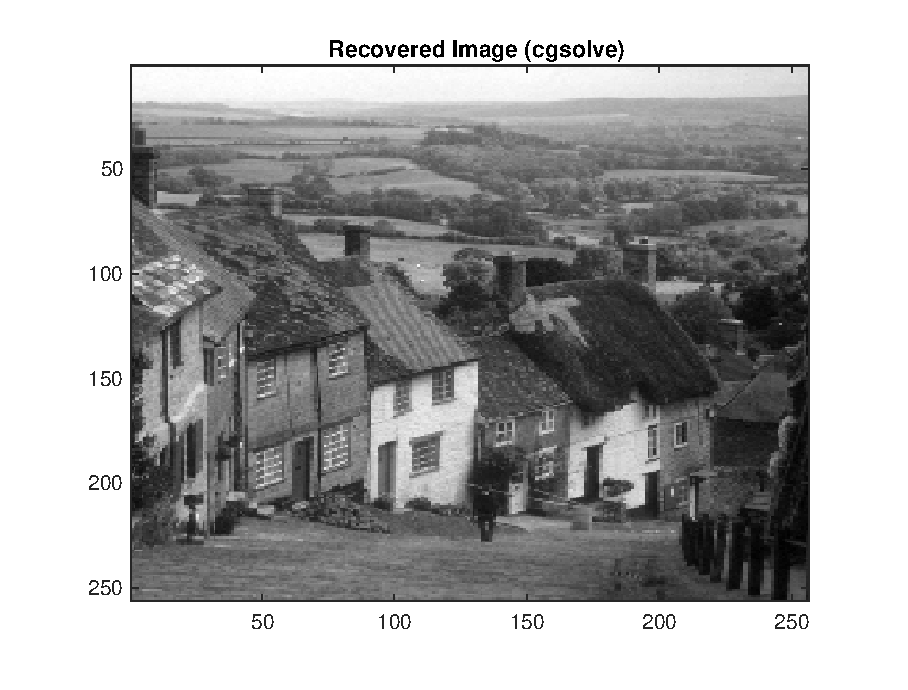
\includegraphics[width=\maxwidth{56.196688409433015em}]{figure_2.eps}
\end{center}
\begin{matlabcode}
fprintf("Original image found in %d steps w/ conjugate gradients\n", iter);
\end{matlabcode}
\begin{matlaboutput}
Original image found in 77 steps w/ conjugate gradients
\end{matlaboutput}

\newpage

\matlabheading{Problem 11.5}

\begin{matlabcode}
function plotFaces(X,numPerLine,numLines)

faceW = 32; 
faceH = 32; 

Y = zeros(faceH*numLines,faceW*numPerLine); 
for i=0:numLines-1 
  	for j=0:numPerLine-1 
    	 Y(i*faceH+1:(i+1)*faceH,j*faceW+1:(j+1)*faceW) = reshape(X(:,i*numPerLine+j+1),[faceH,faceW]); 
  	end 
end 

figure()
imagesc(Y);
colormap(gray);
axis off;
axis equal;
end
\end{matlabcode}

\begin{par}
\begin{flushleft}
\textit{Part A} - Write a function to find the optimal affine approximation to the data in faces:
\end{flushleft}
\end{par}

\begin{matlabcode}
function [Q, theta] = myPCA(X, r)
    sample_mean = mean(X, 2);
    x_tilde = X - sample_mean;
    [Q, ~, ~] = svd(x_tilde);
    Q = Q(:, 1:r);
    theta = Q'*x_tilde(:, 1:r);
end
\end{matlabcode}

\begin{par}
\begin{flushleft}
Plot original 16 faces along with the approximation:
\end{flushleft}
\end{par}

\begin{matlabcode}
load faces

plotFaces(faces, 4, 4); title("First 16 Faces");
\end{matlabcode}
\begin{center}
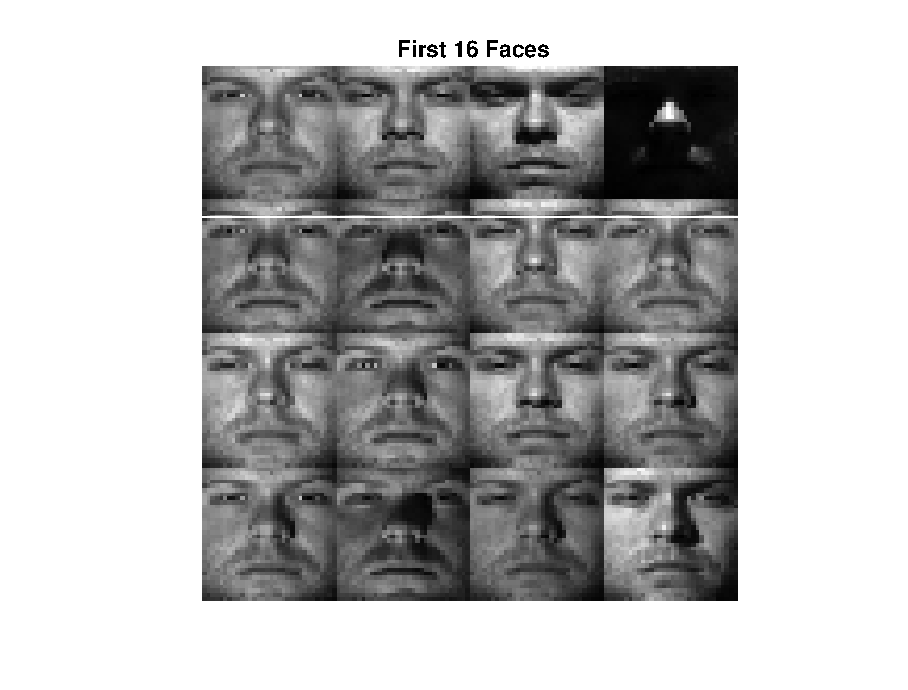
\includegraphics[width=\maxwidth{56.196688409433015em}]{figure_3.eps}
\end{center}
\begin{matlabcode}

r = 16;
[Q, theta] = myPCA(faces, r);
x_hat = sample_mean + Q * theta;
plotFaces(x_hat, 4, 4); title("Approximation of First 16 Faces (r=16)");
\end{matlabcode}
\begin{center}
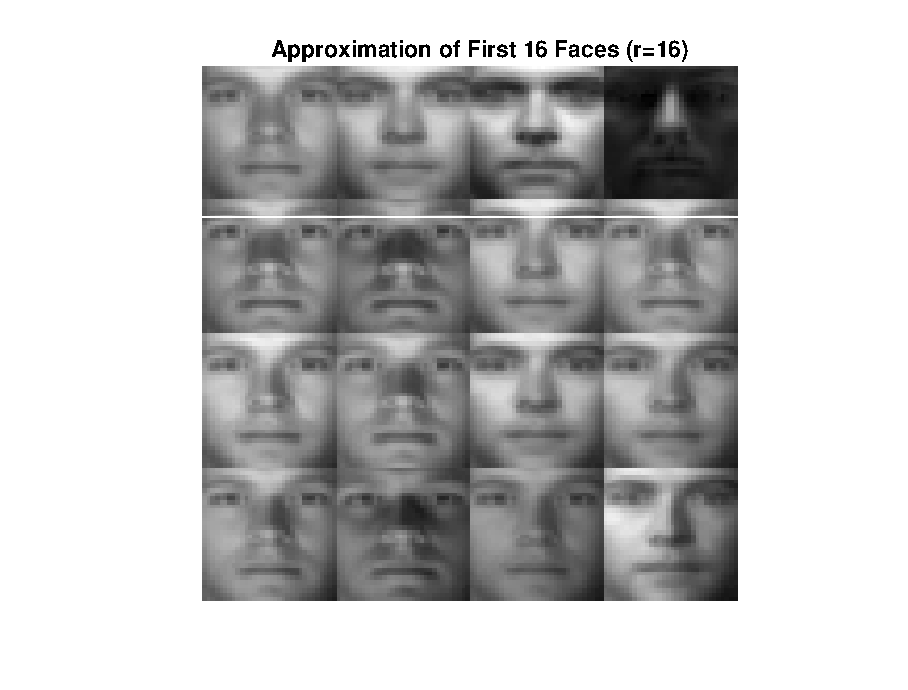
\includegraphics[width=\maxwidth{56.196688409433015em}]{figure_4.eps}
\end{center}


\begin{par}
\begin{flushleft}
\textit{Part B} - Plot each of the basis vectors identified in Part A:
\end{flushleft}
\end{par}

\begin{matlabcode}
plotFaces(Q, 4, 4); title("Basis Vectors from Part A");
\end{matlabcode}
\begin{center}
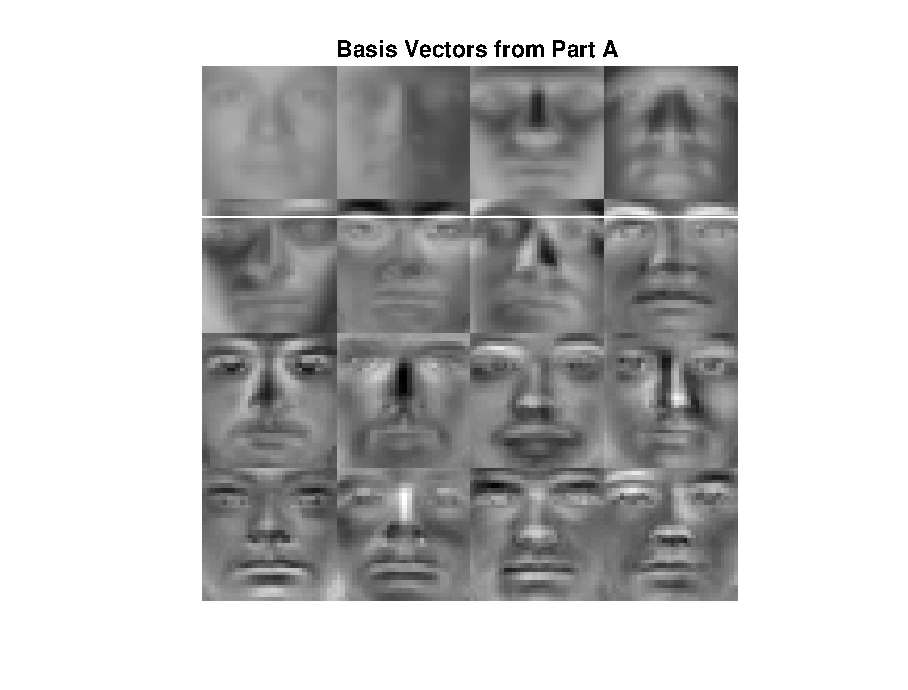
\includegraphics[width=\maxwidth{56.196688409433015em}]{figure_5.eps}
\end{center}


\begin{par}
\begin{flushleft}
\textit{Part C} - Determine the minimum value of r such that the relative error is less than 5 percent:
\end{flushleft}
\end{par}

\begin{par}
\begin{flushleft}
To maintain an error less than 5 percent, r must be greater than or equal to 190. This means that the first 190 singular values of faces account for 95\% of the features in the first 16 entries.
\end{flushleft}
\end{par}

\begin{matlabcode}
for i = 16:2414
    [Q, theta] = myPCA(faces, i);
    x_hat = sample_mean + Q * theta;
    if (norm(x_hat(:, 1:16) - faces(:, 1:16), 'fro')/norm(faces(:, 1:16), 'fro') * 100 < 5)
        break;
    end
end
fprintf("Minimum value of r such that relative error is less than 5 percent: %d", i);
\end{matlabcode}
\begin{matlaboutput}
Minimum value of r such that relative error is less than 5 percent: 190
\end{matlaboutput}


\begin{par}
\begin{flushleft}
\textit{Part D} - Comment on the qualitiative differences between the original dataset and the approximation as r varies:
\end{flushleft}
\end{par}

\begin{par}
\begin{flushleft}
The larger r is, the more accurate the approximation gets. As r decreases, the approximations become more smooth, appearing like an average of all of the faces. Only the particularly prominant "face-like" features are captured in the approximation.
\end{flushleft}
\end{par}

\end{document}
